
\typeout{IJCAI-11 Instructions for Authors}

% These are the instructions for authors for IJCAI-11.
% They are the same as the ones for IJCAI-07 with superficical wording
%   changes only.

\documentclass{article}
% The file ijcai11.sty is the style file for IJCAI-11 (same as ijcai07.sty).
\usepackage{ijcai11}

% Use the postscript times font!
\usepackage{times}

\usepackage{hyperref}
\usepackage{amsmath}
\usepackage{amssymb}
\usepackage{graphicx}
\usepackage{complexity}

% the following package is optional:
%\usepackage{latexsym} 

% Following comment is from ijcai97-submit.tex:
% The preparation of these files was supported by Schlumberger Palo Alto
% Research, AT\&T Bell Laboratories, and Morgan Kaufmann Publishers.
% Shirley Jowell, of Morgan Kaufmann Publishers, and Peter F.
% Patel-Schneider, of AT\&T Bell Laboratories collaborated on their
% preparation.

% These instructions can be modified and used in other conferences as long
% as credit to the authors and supporting agencies is retained, this notice
% is not changed, and further modification or reuse is not restricted.
% Neither Shirley Jowell nor Peter F. Patel-Schneider can be listed as
% contacts for providing assistance without their prior permission.

% To use for other conferences, change references to files and the
% conference appropriate and use other authors, contacts, publishers, and
% organizations.
% Also change the deadline and address for returning papers and the length and
% page charge instructions.
% Put where the files are available in the appropriate places.


\title{The Reusability of zk-SNARKs in the Zcash Protocol}
%\thanks{These match the formatting instructions of IJCAI-07. The support of IJCAI, Inc. is acknowledged.}}
\author{Cordian A. Daniluk \\ 
Laboratoire Jean Kuntzmann\\
Grenoble, France \\
cordian.daniluk@grenoble-inp.org \\
\\
Supervised by: Aude Maignan} % Mosig student

\begin{document}




\maketitle

{% Mosig student
  {\hbox to0pt{\vbox{\baselineskip=10dd\hrule\hbox
to\hsize{\vrule\kern3pt\vbox{\kern3pt
\hbox{{\small I understand what plagiarism entails and I declare that this report }}
\hbox{{\small is my own, original work. }}
\hbox{{\small Cordian A. Daniluk, March 30th, 2022:}}
\kern3pt
}\hfil%\kern3pt
\vrule
}\hrule}
}}
}

\begin{abstract}
        something
\end{abstract}

\section{Introduction}

Cryptocurrencies such as Bitcoin \cite{nakamoto:bitcoin} were designed with the goal to decentralize money transfer.
There should not be a central trusted party such as a bank, through which passes every transaction to remove the need for trust.
However, without any trusted party, transactions are not checked for validity such as the fact that a spender must really be the owner of the spent money and that a spender cannot spend money twice.

A commonly used solution by cryptocurrencies to enforce these rules and yet others is a public ledger called the blockchain \cite{nakamoto:bitcoin}.
The public nature of this data structure enables any node in the cryptocurrency's network to verify rules such as ownership of spent money or double spending money.
However, without appropriate measures a public ledger can lead to compromised privacy by revealing information such as the identities of transaction participants.
In the special case of Bitcoin, a spent amount of money is associated with a destination address, effectively a user's pseudonym.
A user may employ an arbitrary number of pseudonyms to hide their true identity and additionally use methods similar to money laundering, but even these fail to guarantee anonymity \cite{reid:bitcoin-anon}.
Hence, people have tried improving anonymity in new cryptocurrencies such as Monero \cite{saberhagen:cryptonote} or Zcash \cite{hopwood:zcash}.
Zcash is the one this internship is focusing on.

Zcash still uses a blockchain, but to make stronger anonymity guarantees than Bitcoin, Zcash offers shielded transactions as well as transparent transactions inherited from Bitcoin.
While the latter leak data such as the pseudonyms of senders and receivers, the former hide it by either encrypting sensitive information on the blockchain in an anonymity-preserving way or not including it at all.
This lack of inclusion needs additional care, however, since classical Bitcoin nodes need some public information such as a sender's pseudonym to enforce the blockchain's validity.
To this end, a cryptographic construct called zero-knowledge succinct non-interactive argument of knowledge (zk-SNARK) is used.
A zk-SNARK has primary and auxiliary inputs.
The former are publicly known, the latter are only known to the sender.
The sender adds all sensitive information as the auxiliary input and some other as the primary input, creates a zk-SNARK from these, and adds it to a shielded transaction.
The zk-SNARK expresses the statement that the sender knows primary and auxiliary inputs such that the transaction is valid, e.g., that the sender rightfully claims ownership of a given amount of money.
Upon inclusion in the blockchain, anyone can verify the zk-SNARK to enforce the transaction's validity.
Hence, nodes do not do this on public data directly included in the blockchain as in Bitcoin, but on a zk-SNARK, which enables validation of transactions without revealing its auxiliary inputs.

The various properties of zk-SNARKs render them useful in Zcash: they are zero-knowledge, meaning that they prove statements on auxiliary inputs without revealing them.
Their succinctness makes for proofs of small size.
Since they are non-interactive, unlike proposed by, for example, the foundational paper of zero-knowledge proofs \cite{goldwasser:zk}, they can be included in the blockchain without further communication between sender and other parties.
Finally, they are arguments, meaning that a malicious, computationally bounded sender cannot fake proofs to mislead nodes in the network.
More specifically, they are arguments of knowledge, which means that not only do auxiliary inputs exist that satisfy the proven statement, but also that the prover knows them.

Beyond its theoretical definition, zk-SNARKs steadily evolve to make them even more practical.
In Zcash alone, three different zk-SNARKs \cite{bensasson:zksnark} \cite{groth:zksnark} \cite{hopwood:zcash} have been used throughout the protocol's history.
While there are many other details in the Zcash protocol to increase anonymity than merely zk-SNARKs, they are the main mechanism.

There might be situations, where the creation of zk-SNARKs does not have to be done from scratch: the network might have rejected a transaction for various reasons (insufficient transaction fee, chain reorganization, unfulfilled consensus rules, etc.) and the user wants to resend the transaction.
This internship will investigate under what circumstances and to what degree the zk-SNARKs in the resent transaction have to be entirely recalculated, modified, or can be left as is.
It will focus on a transaction type called JoinSplit that has been in Zcash ever since its very first version called Sprout.
The used zk-SNARK is Groth16 \cite{groth:zksnark}, which is used since the Sapling network upgrade.
Additionally, resending will only be considered for transactions sent by a Zcash full node on that same node.
Lightweight clients are also of interest, but introduce further complications that are not related to the recalculation of the zk-SNARK.

The report is structured as follows: first, some background information is given on transactions in Zcash, focusing on JoinSplit descriptions and the Groth16 zk-SNARK.
Next, the various steps needed to resend a refused transaction are outlined and explained.
The focus here is on the recreation of the zk-SNARK.
Once the theory has been covered, a performance comparison of fully recalculating a zk-SNARK and optimized recalculations in various scenarios are be performed.
The report finishes with a conclusion of the work done and suggestions for future work.

%- only TX sent by non-mining full nodes; lightweight clients might also benefit, but not considered for now
%- timeline: send TX to peers -> TX refused -> check what fields need change -> recalculate fields -> resend TX to peers
%- TX refused: need way to detect TX refusal by using timeout (delay of TX inclusion into chain must be short) and confirmation (TX must be confirmed by 6 blocks). several ways to find "current" blockchain:
%        - locally: keep track of transactions in zcashd, remove once fully confirmed (TX has 6 confirmations in local blockchain, e.g.)
%        (- externally: use external tools such as chain explorers (or local zcashd via zmq?) to track transactions)
%  in any case, once refusal detected, resending finally happens via local node. locally by calling a function, externally by invoking an RPC command.
%- check what fields need change: fields designate TX elements + auxiliary inputs (primary ones are subset of TX); dependencies between fields exist, so fields change directly or indirectly.
%  given a dependency graph (with additional conditions on branches), need to determine directly changed ones according to the reason for TX refusal
%- recalculate fields: all fields that change, as found in the previous step, must be recalculated:
%        - if none change, nothing to be done.
%        - if only transaction fields that are not inputs to the proof change, adjust them.
%        - if inputs to the proof change
%- resent TX to peers: the local node resends the TX to its peers
%- NOTE: some steps could partially be implemented externally, but we will assume that everything is done locally.

% explain TX and JoinSplit descriptions
\section{Transactions in Sprout}

Transactions in Sprout consist of transparent inputs and outputs, as well as JoinSplit descriptions.

\subsection{JoinSplit Descriptions}

\begin{figure}[t]
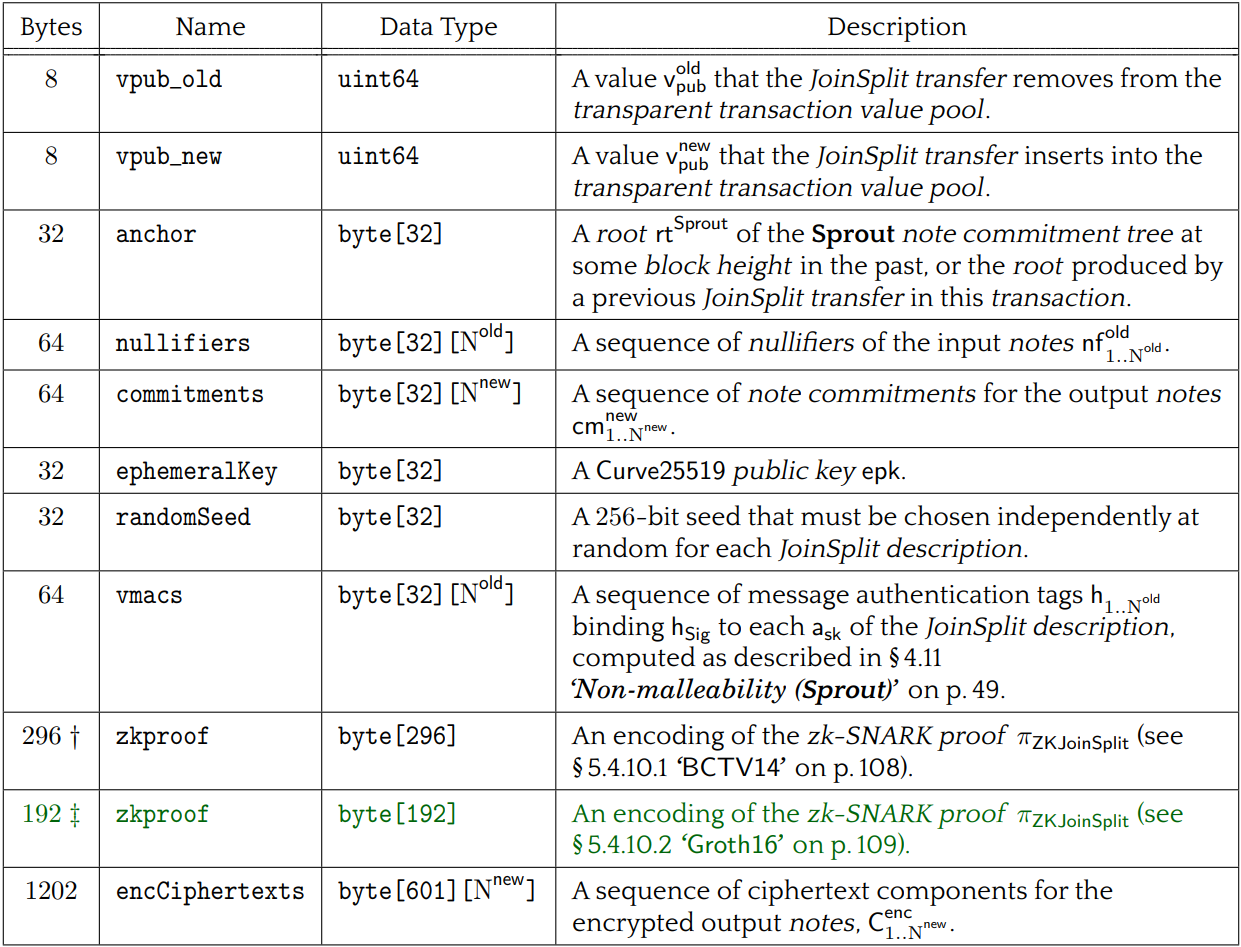
\includegraphics[width=8cm]{images/joinsplit.png}
\caption{A JoinSplit description.} \label{fig:joinsplit}
\centering
\end{figure}

\begin{figure}[t]
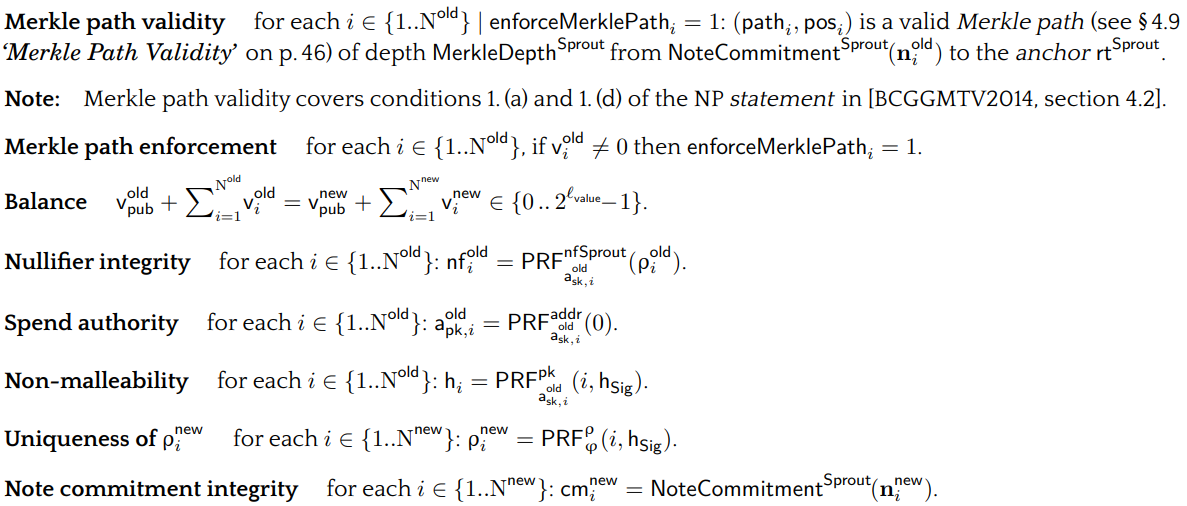
\includegraphics[width=8.5cm]{images/proofconditions.png}
\caption{Conditions validated by the proof.} \label{fig:joinsplit}
\centering
\end{figure}

\subsection{The Groth16 zk-SNARK}

The Groth16 proving system provides a way to prove statements of the form $x \in L$ where $L \in \NP$.
For Zcash, $x$ would be chosen parts of a JoinSplit and $L$ is the statement ``$x$ is a valid JoinSplit''.
In this section, we will show informally how a zk-SNARK is produced from such a statement $x \in L$.

Fix a language $L \subseteq \NP$.
Then, there exists an algorithm $A(x, w)$ polynomial in $|x|$ such that

\begin{align*} L = \{ x \mid \exists w\colon A(x, w) = 0\} \end{align*}

Now, define ARITH-SAT to be the following language:

\begin{align*} \text{ARITH-SAT} := \{ \text{An arithmetic circuit } C \mid \exists w\colon C(w) = 0\} \end{align*}

$C(w)$ represents the output of $C$ if wires are assigned the values in $w$.
ARITH-SAT is \NP-complete (similarly to how 3-SAT is \NP-complete), so $L \leq_p \text{ARITH-SAT}$ and $L$ can be efficiently converted into a more general form $C$.

Let $m$ be the number of wires of $C$, including inputs.
For $k$ multiplication gates in $C$, choose $r_1, \ldots, r_k$ pairwise distinct in $\mathbb{F}$.
Set $t(x) = \prod_{i=1}^k(x-r_i)$.


Next, define a quadratic arithmetic program (QAP) $Q := (\{u_i \in \mathbb{F}[x] \mid i \in [m]\}, \{v_i \in \mathbb{F}[x] \mid i \in [m]\}, \{w_i \in \mathbb{F}[x] \mid i \in [m]\}, t)$ that computes an arithmetic circuit $C$ if

\begin{align*}
        t(x) \mid \sum_{i=0}^m a_iu_i(x) \cdot \sum_{i=0}^m a_iv_i(x) - \sum_{i=0}^{m} a_iw_i(x)
\end{align*}

Intuitively, $L(r_j) := \sum_{i=0}^m a_iu_i(r_j)$ corresponds to the left input of the multiplication gate associated with $r_j$,
$R(r_j) := \sum_{i=0}^m a_iv_i(r_j)$ is its right input and $O(r_j) := \sum_{i=0}^{m} a_iw_i(x)$ its output.
If $L(r_j)R(r_j) - O(r_j) = 0$, then the wires have been assigned values that correspond to the circuit structure.
In order to ensure this for all $r_j$, divisibility by $t$ is required.

% TODO: formal definition of zk-SNARK????

Given $Q$, we can now calculate the proof. Let $G_1, G_2$ be two cyclic groups with generators $g_1, g_2$, respectively.
Then, the proof $\pi$ for the statement $x \in L$ is $\pi := (g_1^A, g_2^B, g_1^C)$, where

\begin{align}
        A &= \alpha + \sum_{i=0}^m a_iu_i(x) + r\delta \\
        B &= \beta + \sum_{i=0}^m a_iv_i(x) + s\delta \\
        C &= \frac{\sum_{i=l+1}^m a_i(\beta u_i(x) + \alpha v_i(x) + w_i(x)) + h(x)t(x)}{\delta} \\
        & + As + Br - rs\delta \nonumber
\end{align}

% explain the timeline: (1) send TX to peers -> (2) TX refused -> (3) check what fields need change -> (4) recalculate fields -> (5) resend TX to peers AND (1), (2), and (5) entirely, (3) and (4) are discussed afterwards
\section{Resending Shielded Transactions}

\begin{figure}[t]

\includegraphics[width=8cm]{images/timeline.png}
\caption{Steps involved in resending a transaction.} \label{fig:resend-steps}
\centering
\end{figure}

We fix the following series of events: a Zcash full node creates and sends a transaction containing a JoinSplit description to its peers.
At some later point, it learns that the transaction has not been included into the blockchain.
The node wants to resend the transaction: it checks what fields need to change, recalculates these and finally resends the transaction.
This process is depicted in Figure \ref{fig:resend-steps}.
It can be repeated until the transaction is in the blockchain.

We assume that the node is capable of sending and resending to an adequate number of peers, such that the physical network does not inhibit the transaction's inclusion.
Hence, we will not deal with the first and the last step of Figure \ref{fig:resend-steps}.
A node can assume that its transaction has been refused by waiting for the transaction's inclusion and then for its confirmation.
If the node does not find its transaction in its local blockchain after some time, the transaction has been refused.
This can happen for insufficient transaction fees, for example.
If it is included, but not fully confirmed by a sufficient number of blocks, it has been refused as well.
This can happen for a chain reorganization, where blocks become stale because another, longer\footnote{Longer not in terms of block length but accumulated block difficulty.} branch has overtaken them.

Once it is certain that a transaction has been refused, it must be checked what fields of the JoinSplit must change to maximize the chances of inclusion.
All JoinSplit fields, which include primary inputs, as well as all auxiliary inputs are listed in two tables in Figure \ref{fig:joinsplit-change} and \ref{fig:proof-change}.

\begin{figure}[t]
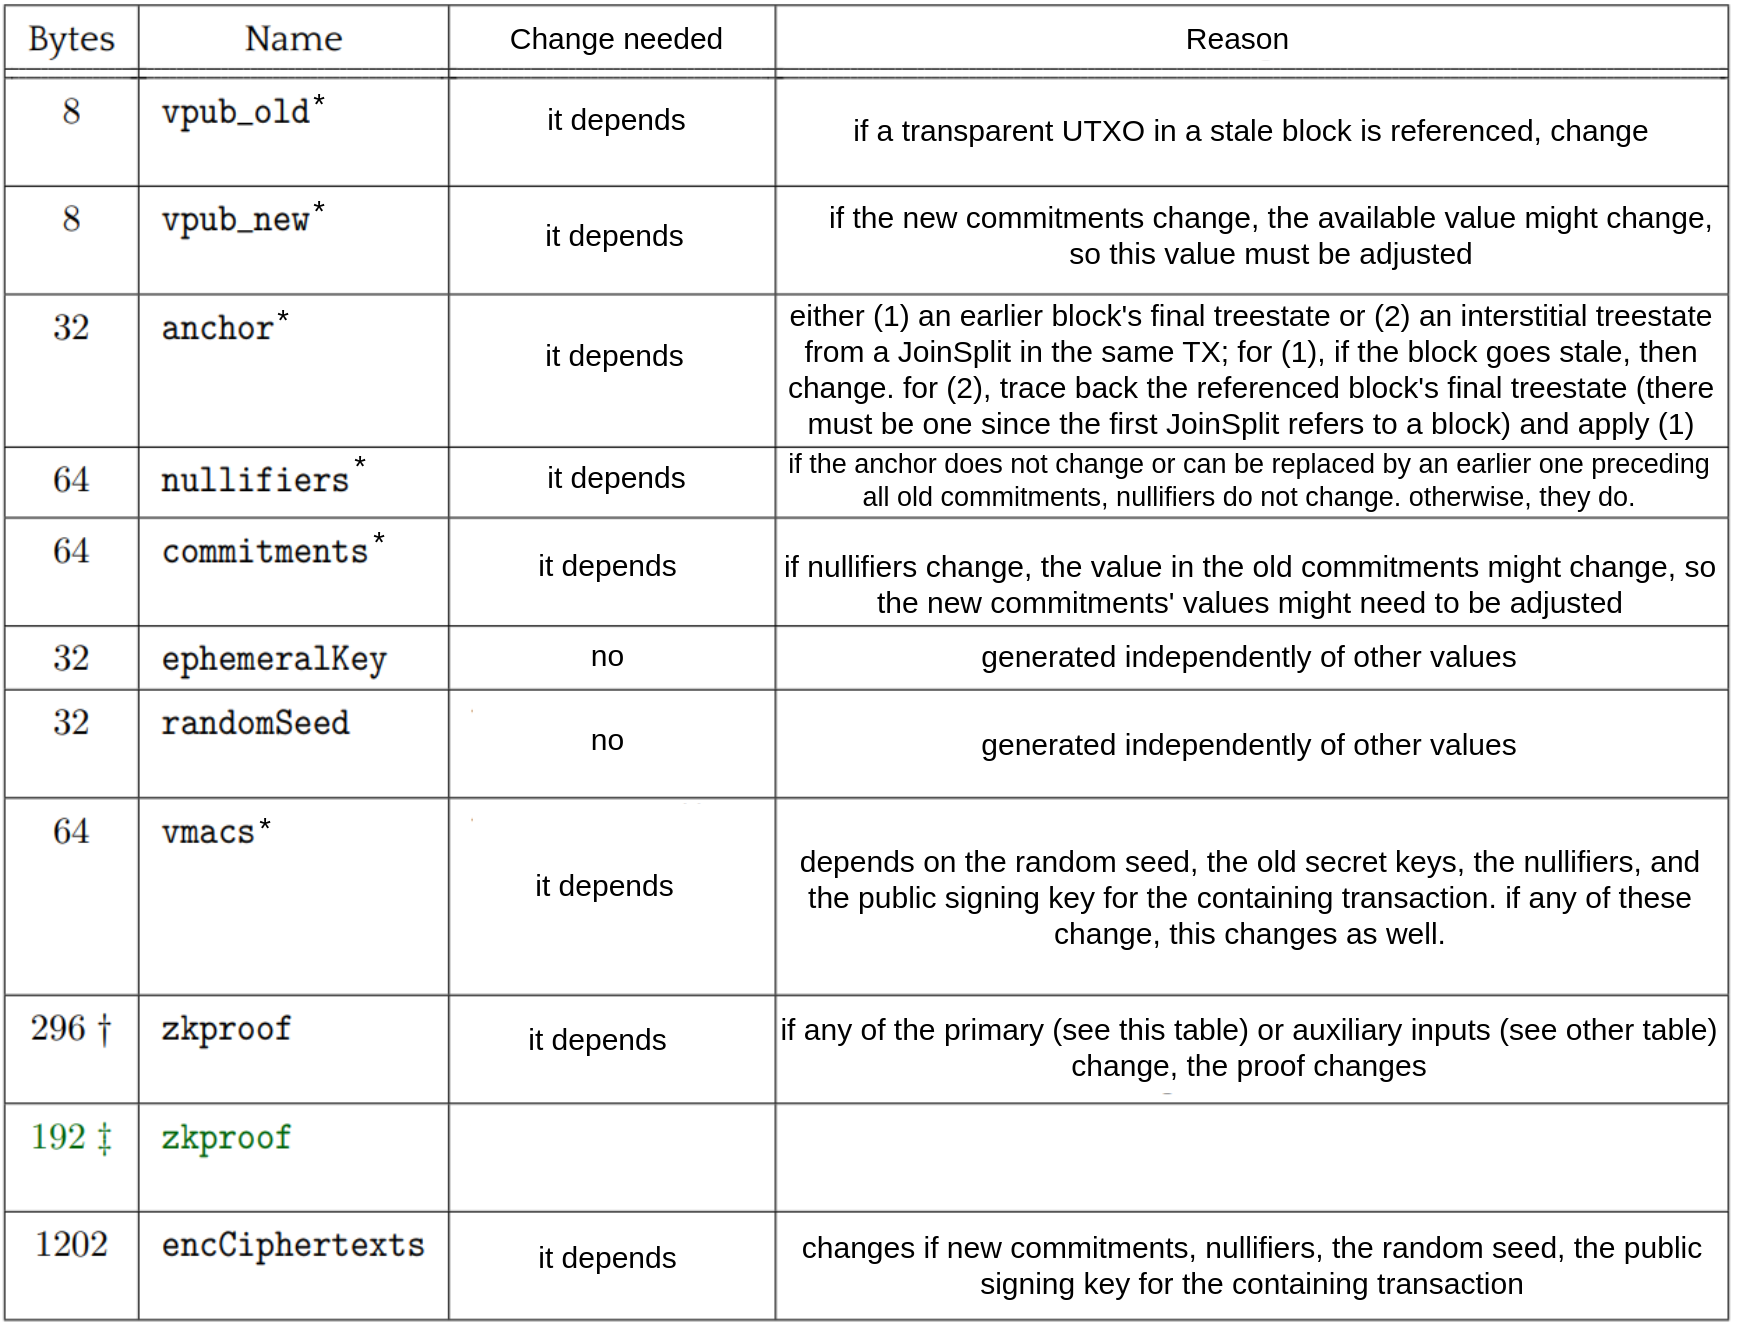
\includegraphics[width=8cm]{images/transactionchange.png}
\caption{All transaction fields, which include primary inputs, with explanations whether they need to change or not.} \label{fig:joinsplit-change}
\centering
\end{figure}

\begin{figure}[t]
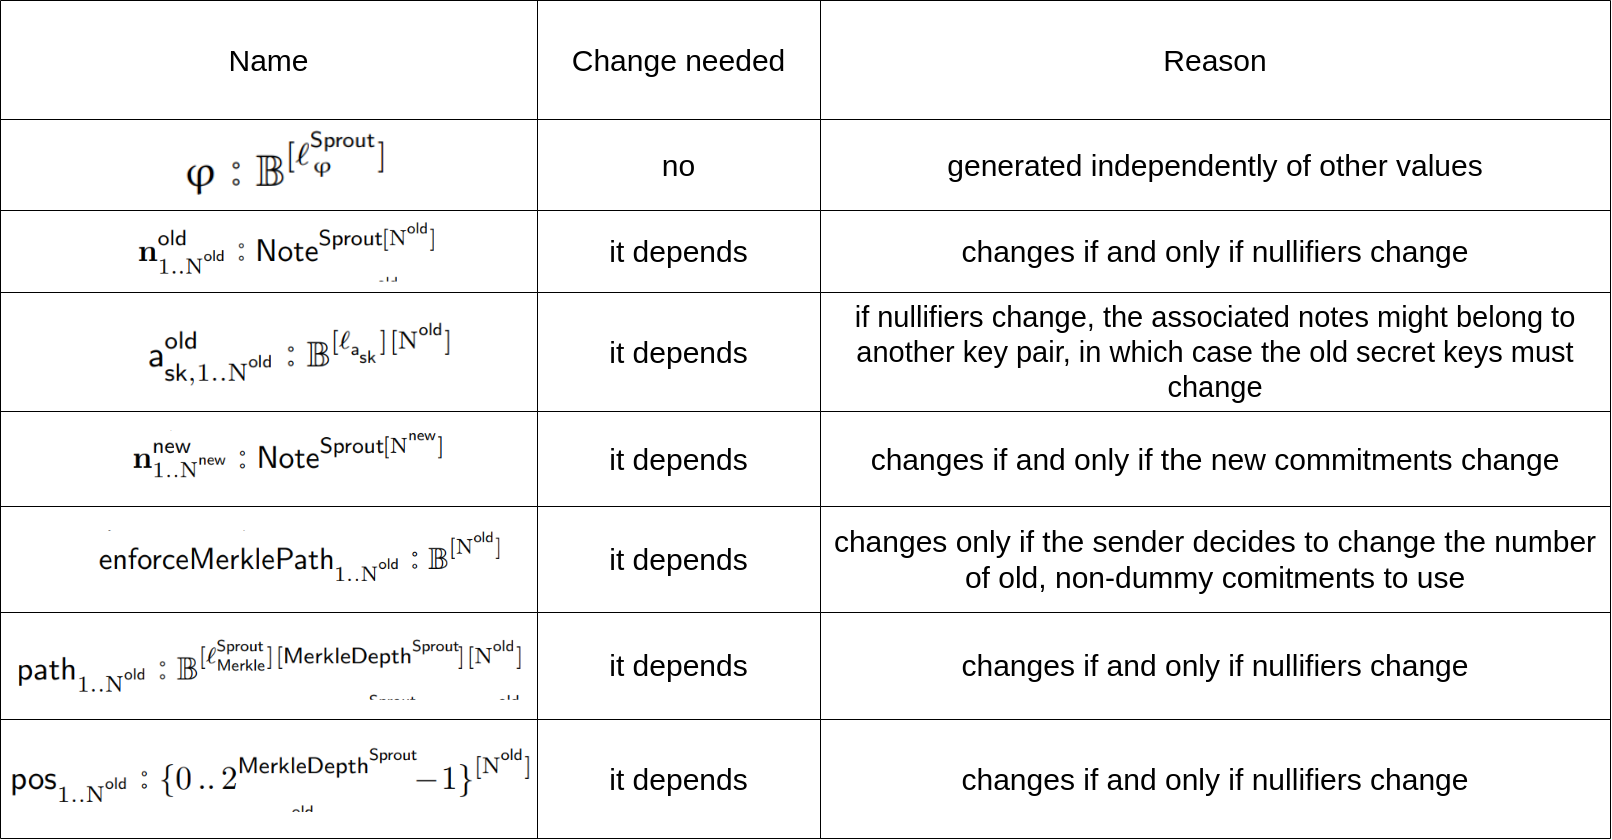
\includegraphics[width=8cm]{images/proofchange.png}
\caption{All auxiliary inputs with explanations whether they need to change or not.} \label{fig:proof-change}
\centering
\end{figure}

\section{Optimizing The zk-SNARK's Recalculation}

what can be doing just knowing the old proof?

apparently not much... what can be done with some more knowledge?

\section{Performance Measurements}

\section{Conclusion}

\section{Outlook}

%\subsection{Length of Papers}
%
%Each accepted full paper is allocated six pages in the conference 
%proceedings. Up to two additional pages may be purchased at a price 
%of \$275 per page for any accepted paper. However, all 
%{\em submissions} must 
%be a maximum of six pages in length.
%
%
%\subsection{Word Processing Software}
%
%As detailed below, IJCAI has prepared and made available a set of
%\LaTeX{} macros and a Microsoft Word template for use in formatting
%your paper. If you are using some other word processing software (such
%as WordPerfect, etc.), please follow the format instructions given
%below and ensure that your final paper looks as much like this sample
%as possible.
%
%\section{Style and Format}
%
%\LaTeX{} and Word style files that implement these instructions
%can be retrieved electronically. (See Appendix~\ref{stylefiles} for
%instructions on how to obtain these files.)
%
%\subsection{Layout}
%
%Print manuscripts two columns to a page, in the manner in which these
%instructions are printed. The exact dimensions for pages are:
%\begin{itemize}
%\item left and right margins: .75$''$
%\item column width: 3.375$''$
%\item gap between columns: .25$''$
%\item top margin---first page: 1.375$''$
%\item top margin---other pages: .75$''$
%\item bottom margin: 1.25$''$
%\item column height---first page: 6.625$''$
%\item column height---other pages: 9$''$
%\end{itemize}
%
%All measurements assume an 8-1/2$''$ $\times$ 11$''$ page size. For
%A4-size paper, use the given top and left margins, column width,
%height, and gap, and modify the bottom and right margins as necessary.
%
%\subsection{Format of Electronic Manuscript}
%
%For the production of the electronic manuscript, you must use Adobe's
%{\em Portable Document Format} (PDF). A PDF file can be generated, for
%instance, on Unix systems using {\tt ps2pdf} or on Windows systems
%using Adobe's Distiller. There is also a website with free software
%and conversion services: {\tt http://www.ps2pdf.com/}. For reasons of
%uniformity, use of Adobe's {\em Times Roman} font is strongly suggested. In
%\LaTeX2e{}, this is accomplished by putting
%\begin{quote} 
%\mbox{\tt $\backslash$usepackage\{times\}}
%\end{quote}
%in the preamble.\footnote{You may want also to use the package {\tt
%latexsym}, which defines all symbols known from the old \LaTeX{}
%version.}
%  
%Additionally, it is of utmost importance to specify the American {\bf
%letter} format (corresponding to 8-1/2$''$ $\times$ 11$''$) when
%formatting the paper. When working with {\tt dvips}, for instance, one
%should specify {\tt -t letter}.
%
%\subsection{Title and Author Information}
%
%Center the title on the entire width of the page in a 14-point bold
%font. Below it, center the author name(s) in a 12-point bold font, and
%then center the address(es) in a 12-point regular font. Credit to a
%sponsoring agency can appear on the first page as a footnote.
%
%\subsubsection{Blind Review}
%
%In order to make blind reviewing possible, authors must omit their
%names and affiliations when submitting the paper for review. In place
%of names and affiliations, provide a list of content areas. When
%referring to one's own work, use the third person rather than the
%first person. For example, say, ``Previously,
%Gottlob~\shortcite{gottlob:nonmon} has shown that\ldots'', rather
%than, ``In our previous work~\cite{gottlob:nonmon}, we have shown
%that\ldots'' Try to avoid including any information in the body of the
%paper or references that would identify the authors or their
%institutions. Such information can be added to the final camera-ready
%version for publication.
%
%\subsection{Abstract}
%
%Place the abstract at the beginning of the first column 3$''$ from the
%top of the page, unless that does not leave enough room for the title
%and author information. Use a slightly smaller width than in the body
%of the paper. Head the abstract with ``Abstract'' centered above the
%body of the abstract in a 12-point bold font. The body of the abstract
%should be in the same font as the body of the paper.
%
%The abstract should be a concise, one-paragraph summary describing the
%general thesis and conclusion of your paper. A reader should be able
%to learn the purpose of the paper and the reason for its importance
%from the abstract. The abstract should be no more than 200 words long.
%
%\subsection{Text}
%
%The main body of the text immediately follows the abstract. Use
%10-point type in a clear, readable font with 1-point leading (10 on
%11).
%
%Indent when starting a new paragraph, except after major headings.
%
%\subsection{Headings and Sections}
%
%When necessary, headings should be used to separate major sections of
%your paper. (These instructions use many headings to demonstrate their
%appearance; your paper should have fewer headings.)
%
%\subsubsection{Section Headings}
%
%Print section headings in 12-point bold type in the style shown in
%these instructions. Leave a blank space of approximately 10 points
%above and 4 points below section headings.  Number sections with
%arabic numerals.
%
%\subsubsection{Subsection Headings}
%
%Print subsection headings in 11-point bold type. Leave a blank space
%of approximately 8 points above and 3 points below subsection
%headings. Number subsections with the section number and the
%subsection number (in arabic numerals) separated by a
%period.
%
%\subsubsection{Subsubsection Headings}
%
%Print subsubsection headings in 10-point bold type. Leave a blank
%space of approximately 6 points above subsubsection headings. Do not
%number subsubsections.
%
%\subsubsection{Special Sections}
%
%You may include an unnumbered acknowledgments section, including
%acknowledgments of help from colleagues, financial support, and
%permission to publish.
%
%Any appendices directly follow the text and look like sections, except
%that they are numbered with capital letters instead of arabic
%numerals.
%
%The references section is headed ``References,'' printed in the same
%style as a section heading but without a number. A sample list of
%references is given at the end of these instructions. Use a consistent
%format for references, such as that provided by Bib\TeX{}. The reference
%list should not include unpublished work.
%
%\subsection{Citations}
%
%Citations within the text should include the author's last name and
%the year of publication, for example~\cite{gottlob:nonmon}.  Append
%lowercase letters to the year in cases of ambiguity.  Treat multiple
%authors as in the following examples:~\cite{abelson-et-al:scheme}
%or~\cite{bgf:Lixto} (for more than two authors) and
%\cite{brachman-schmolze:kl-one} (for two authors).  If the author
%portion of a citation is obvious, omit it, e.g.,
%Nebel~\shortcite{nebel:jair-2000}.  Collapse multiple citations as
%follows:~\cite{gls:hypertrees,levesque:functional-foundations}.
%\nocite{abelson-et-al:scheme}
%\nocite{bgf:Lixto}
%\nocite{brachman-schmolze:kl-one}
%\nocite{gottlob:nonmon}
%\nocite{gls:hypertrees}
%\nocite{levesque:functional-foundations}
%\nocite{levesque:belief}
%\nocite{nebel:jair-2000}
%
%\subsection{Footnotes}
%
%Place footnotes at the bottom of the page in a 9-point font.  Refer to
%them with superscript numbers.\footnote{This is how your footnotes
%should appear.} Separate them from the text by a short
%line.\footnote{Note the line separating these footnotes from the
%text.} Avoid footnotes as much as possible; they interrupt the flow of
%the text.
%
%\section{Illustrations}
%
%Place all illustrations (figures, drawings, tables, and photographs)
%throughout the paper at the places where they are first discussed,
%rather than at the end of the paper. If placed at the bottom or top of
%a page, illustrations may run across both columns.
%
%Illustrations must be rendered electronically or scanned and placed
%directly in your document. All illustrations should be in black and
%white, as color illustrations may cause problems. Line weights should
%be 1/2-point or thicker. Avoid screens and superimposing type on
%patterns as these effects may not reproduce well.
%
%Number illustrations sequentially. Use references of the following
%form: Figure 1, Table 2, etc. Place illustration numbers and captions
%under illustrations. Leave a margin of 1/4-inch around the area
%covered by the illustration and caption.  Use 9-point type for
%captions, labels, and other text in illustrations.
%
%\section*{Acknowledgments}
%
%The preparation of these instructions and the \LaTeX{} and Bib\TeX{}
%files that implement them was supported by Schlumberger Palo Alto
%Research, AT\&T Bell Laboratories, and Morgan Kaufmann Publishers.
%Preparation of the Microsoft Word file was supported by IJCAI.  An
%early version of this document was created by Shirley Jowell and Peter
%F. Patel-Schneider.  It was subsequently modified by Jennifer
%Ballentine and Thomas Dean, Bernhard Nebel, and Daniel Pagenstecher.
%These instructions are the same as the ones for IJCAI--05, prepared by
%Kurt Steinkraus, Massachusetts Institute of Technology, Computer
%Science and Artificial Intelligence Lab.
%
%\appendix
%
%\section{\LaTeX{} and Word Style Files}\label{stylefiles}
%
%The \LaTeX{} and Word style files are available on the IJCAI--11
%website, {\tt http://www.ijcai-11.org/}.
%These style files implement the formatting instructions in this
%document.
%
%The \LaTeX{} files are {\tt ijcai11.sty} and {\tt ijcai11.tex}, and
%the Bib\TeX{} files are {\tt named.bst} and {\tt ijcai11.bib}. The
%\LaTeX{} style file is for version 2e of \LaTeX{}, and the Bib\TeX{}
%style file is for version 0.99c of Bib\TeX{} ({\em not} version
%0.98i). The {\tt ijcai11.sty} file is the same as the {\tt
%ijcai07.sty} file used for IJCAI--07.
%
%The Microsoft Word style file consists of a single file, {\tt
%ijcai11.doc}. This template is the same as the one used for
%IJCAI--07.
%
%These Microsoft Word and \LaTeX{} files contain the source of the
%present document and may serve as a formatting sample.  
%
%Further information on using these styles for the preparation of
%papers for IJCAI--11 can be obtained by contacting {\tt
%pcchair11@ijcai.org}.

%% The file named.bst is a bibliography style file for BibTeX 0.99c
\bibliographystyle{named}
\bibliography{../bib}

\end{document}

